Before proceeding to the analysis of natural oscillations in twisted string actuators, we would like to start with a brief overview of the mathematical modeling of TSA. For a deeper insight and peculiarities of TSA modeling, the reader may refer to previously published works \cite{nedelchev2020accurate}, \cite{popov2012study}, \cite{palli2012modeling}.

\subsection{Kinematics}
% \subsubsection*{Mathematical Model of a TSA}




According to the conventional representation of a section of twisted string shown in Fig. \ref{fig:schematic_diagram}(a), a cable of length $L$ and radius $r$, twisted at an angle $\theta$, forms a helix and contracts by the $X$ amount. For the resulting right triangle with the sides $(L-X),\theta r$, and $L$ one can derive the geometric constraint of twisted string as:
\begin{equation}\label{eq.mod:geom_const}
\theta^2 r^2 + (L-X)^2 - L^2 = 0  
\end{equation}

It is important to note here that equation above is a second order polynomial, and there exist two solutions for motor angle $\theta$ that correspond to \textit{the same contraction level} $X$.

Differentiating the constraint above yields the relationships between the payload (output) and motor (input) velocities:
\begin{equation}\label{eq.mod:x_dot}
\dot{X} = \mathcal{J}(\theta, X)\dot{\theta}
\end{equation}
where $J$ denotes the Jacobian of twisted strings and $\dot{\theta}$ stands for angular speed. Hereinafter, we will omit the arguments $(\theta, X)$ for the sake of brevity.


It is worth noting that the twisted strings Jacobian may be represented in various ways, depending on the availability of motor or payload variables:
\begin{equation}\label{eq.mod:jacobian}
    \mathcal{J} = \frac{\theta r^2}{L-X} = \frac{\theta r^2}{\sqrt{L^2 - \theta^2 r^2}} = \frac{r \sqrt{L^2 - (L -X)^2}}{L-X} 
\end{equation}

\subsection{Energy}
Total energy of TSA can be represented just like that of any conventional mechanical system as a sum of kinetic, potential and dissipated energy terms $E = E_K + E_P + E_D$ as follows:
\begin{equation}\label{eq.mod:total_energy}
    E = \frac{1}{2} I\dot{\theta}^2 + \frac{1}{2}m \dot{X}^2 + mgX + E_D
\end{equation}
where the first term represents kinetic energy of the spinning motor shaft with inertia $I$, the next two terms correspond to kinetic energy of the payload of mass $m$ moving at speed $\dot{X}$ and its potential energy due to gravity (here we assume the payload always moves along the vertical axis), with $g$ denoting the gravitational constant, while the term $E_D$ represents all the energy losses due to friction inside the motor, payload's sliders and the strings themselves, as well as reflecting all other internal and external disruptive forces, otherwise unaccounted for explicitly.


\begin{figure}
		\centering
		\vspace*{2mm} 
		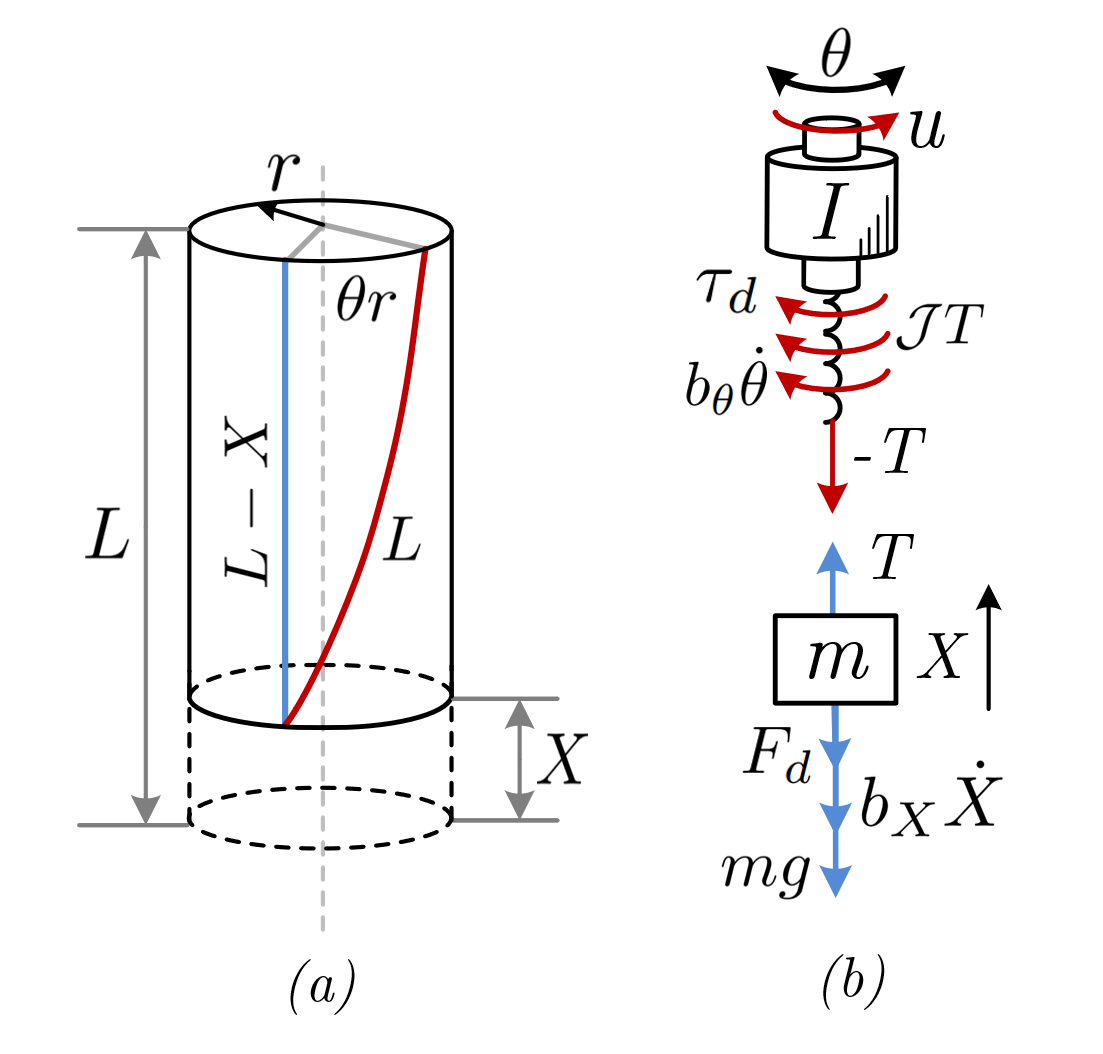
\includegraphics[trim= 0.0cm 1.0cm 0.0cm 0.0cm,width=0.72\columnwidth]{pics/tsa_scheme.PNG}
		\caption{Schematic diagrams for the analysis of TSA kinematics (a) and dynamics (b)}
		\label{fig:schematic_diagram}
\end{figure}
Depending on the variables of choice, one may represent the kinetic and potential energy with the motor-side or payload-side variables using the kinematical constraints \eqref{eq.mod:x_dot} and \eqref{eq.mod:jacobian} as follows:
\begin{equation}\label{eq.mod:K_Pi_energies}
\begin{matrix}
    E_K = \frac{1}{2} (I + m \mathcal{J}^2)\dot{\theta}^2 = \frac{1}{2} (I\mathcal{J}^{-2} + m )\dot{X}^2 \\ 
    \\
    E_P = mgX = mg (L - \sqrt{L^2 - \theta^2r^2} )  \\ 
\end{matrix}
\end{equation}
where terms preceding the squares of velocities $\dot{\theta}^2, \dot{X}^2$ represent the reflected inertia values on the motor and payload sides, respectively. 

\subsection{Dynamics}
A schematic diagram of a twisted string actuator with a connected payload is shown in Fig. \ref{fig:schematic_diagram} (b). After driving the energy equations, one may use Lagrange-Euler approach to derive the equations of motion (EoM) of twisted string actuators as follows:
\begin{equation}\label{eq.mod:dyn_model}
\left\{\begin{matrix}
u = I \ddot{\theta} + \mathcal{J}T  + b_\theta \dot{\theta} + \tau_{d}
\\[0.5em]
T = m \ddot{X} + mg  + b_X \dot{X} + F_{d}
\end{matrix}\right.
\end{equation}
where $u$ denotes motor torque, $T$ stands for string's tension, the terms $ b_\theta,  b_X$ represent viscous friction coefficients in motor and payload, respectively, while the terms $\tau_{d}, F_{d}$ represent the collective effects of all other forces at play inside the TSA system such as dry friction, string jamming and external disturbance applied to the payload. For more information and details on derivation of these forces and particularly ones responsible for losses due to intrinsic string compliance one may refer to our previous work \cite{nedelchev2020accurate}. 

Assuming that the constraint \eqref{eq.mod:geom_const} always holds, one may rewrite the EoM above with respect to motor acceleration as follows:
\begin{equation}\label{eq.mod:dyn_motor}
u = D_\theta (\mathbf{q}) \ddot{\theta} + h_\theta(\mathbf{q},\dot{\mathbf{q}})
\end{equation}
where
\begin{equation*}
\begin{matrix}
D_\theta = I + m \mathcal{J}^2\\
h_\theta = \big(b_\theta + \mathcal{J}(m\dot{\mathcal{J}}+b_X)\big)\dot{\theta} + \mathcal{J}(mg  + F_{d}) + \tau_d
\end{matrix}
\end{equation*}
and $\mathbf{q}$ is the chosen set of generalized coordinates, which may be either one of the motor- and payload-side variables ($\theta$ and $X$, respectively) or both of them, depending on the model used to calculate the Jacobian with \eqref{eq.mod:jacobian}. 

Just like in the case when driving the energy equations, one may use the TSA kinematic model to rewrite the dynamics in terms of the payload acceleration:
\begin{equation}\label{eq.mod:dyn_load}
u = D_X(\mathbf{q}) \ddot{X} + h_X(\mathbf{q},\dot{\mathbf{q}})
\end{equation}
with the dynamical terms $D_X,h_X$ defined as follows:
\begin{equation*}
\begin{matrix}
D_X = I\mathcal{J}^{-2} + m\\
h_X = \big(\mathcal{J}^{-1} b_\theta + \mathcal{J}^{-2} \dot{\mathcal{J}}I + b_X  \big)\dot{X} + \mathcal{J}(mg  + F_{d}) + \tau_d
\end{matrix}
\end{equation*}

Having driven all the necessary dynamical and energy equations, we now move onto the analysis of energy exchange within a TSA system, and in particular, of that in its behavior in the singular configuration. 



\subsection{The Singular Point}
It should be noted that if one is willing to use the kinetic energy model derived in terms of the payload variables, a problem with Jacobian singularity may arise (when $\theta = 0$, $\mathcal{J} = 0$ as suggested by \eqref{eq.mod:jacobian}), which is also the case for the dynamical model \eqref{eq.mod:dyn_load}. Thus, it may naturally seem that this singular configuration ($\theta = 0$) should be avoided at all costs in the applications involving TSA control, unless this is practically impossible. 

From the physical standpoint, the singular configuration corresponds to the fully untwisted state of the strings, which makes is impossible to generate the payload motion (contraction speed $\dot{X}$ is zero regardless of motor specifications). As an immediate consequence, this implies that all mechanical energy of the system in the singularity point can be only stored (and dissipated by) in the motor shaft, since all other sources of energy are zero (no torsional energy accumulated since the strings are untwisted, zero payload-side potential energy since $X=0$ and kinetic energy). In addition, any external force applied to the payload will not affect the motor torque $u$ since the Jacobian is zero. All of these imply that, if there is some kinetic energy within the system in its singular configuration stored due to the motor's inertia, a part of it will be dissipated while the remainder will be converted into other types of energy, e.g. into the kinetic and potential energy of the payload. Thus, the peaks of various energy components contributed by the motor and the payload will be occurring at different time instances. 

One can see simulated energy curves as a function of time in Fig. \ref{fig:energies_simulation}, which were generated after the strings were twisted and then released with zero control effort from the motor side. The string parameters were chosen to be $L$ = 170 mm, $R$ = 0.75 mm. We have introduced non-zero energy dissipation on the motor side to make the simulation more realistic, and one can note in the figure that the total energy levels decrease with time. 
\begin{figure}
		\centering
		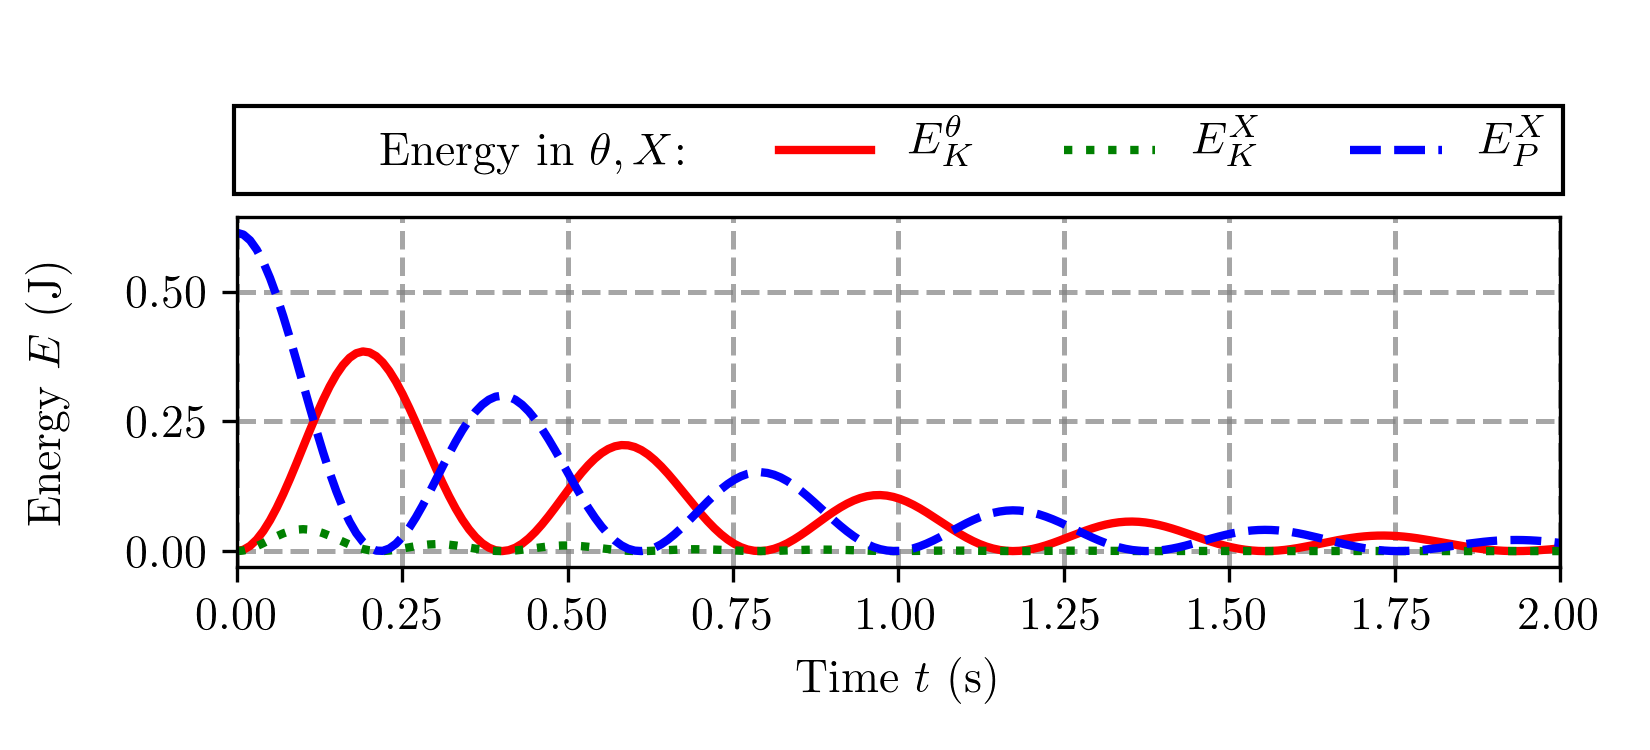
\includegraphics[trim= 0.0cm 0.8cm 0.0cm 0.0cm,width=1.0\columnwidth]{pics/plots/energy_damp.png}
		\caption{Simulated time plot of energy components: kinetic energy of the motor ($E_K^\theta$), payload ($E_K^X$) and potential energy of the latter ($E_P^X$)} 
 		\label{fig:energies_simulation}
		\vspace*{-2mm} 
\end{figure}


It follows from the simulation results that, unless energy dissipation is excessively large, one should be able to observe periodical motion of the system in the phase plane of actuator coordinates $\{\theta, \dot{\theta}\}$ and payload coordinates $\{X,\dot{X}\}$. Moreover, the phase trajectory in the motor space should theoretically lie in all four quadrants of the phase plane, while the payload's phase trajectory must be fully contained on the right hand side of the phase plane (since solution of \eqref{eq.mod:geom_const} with respect to $X$ is always positive) and pass through the origin $X = 0 , \dot{X} = 0$. Simulated phase plots are shown in Fig. \ref{fig:phase_plots_simulation}.

\begin{figure}
		\centering
		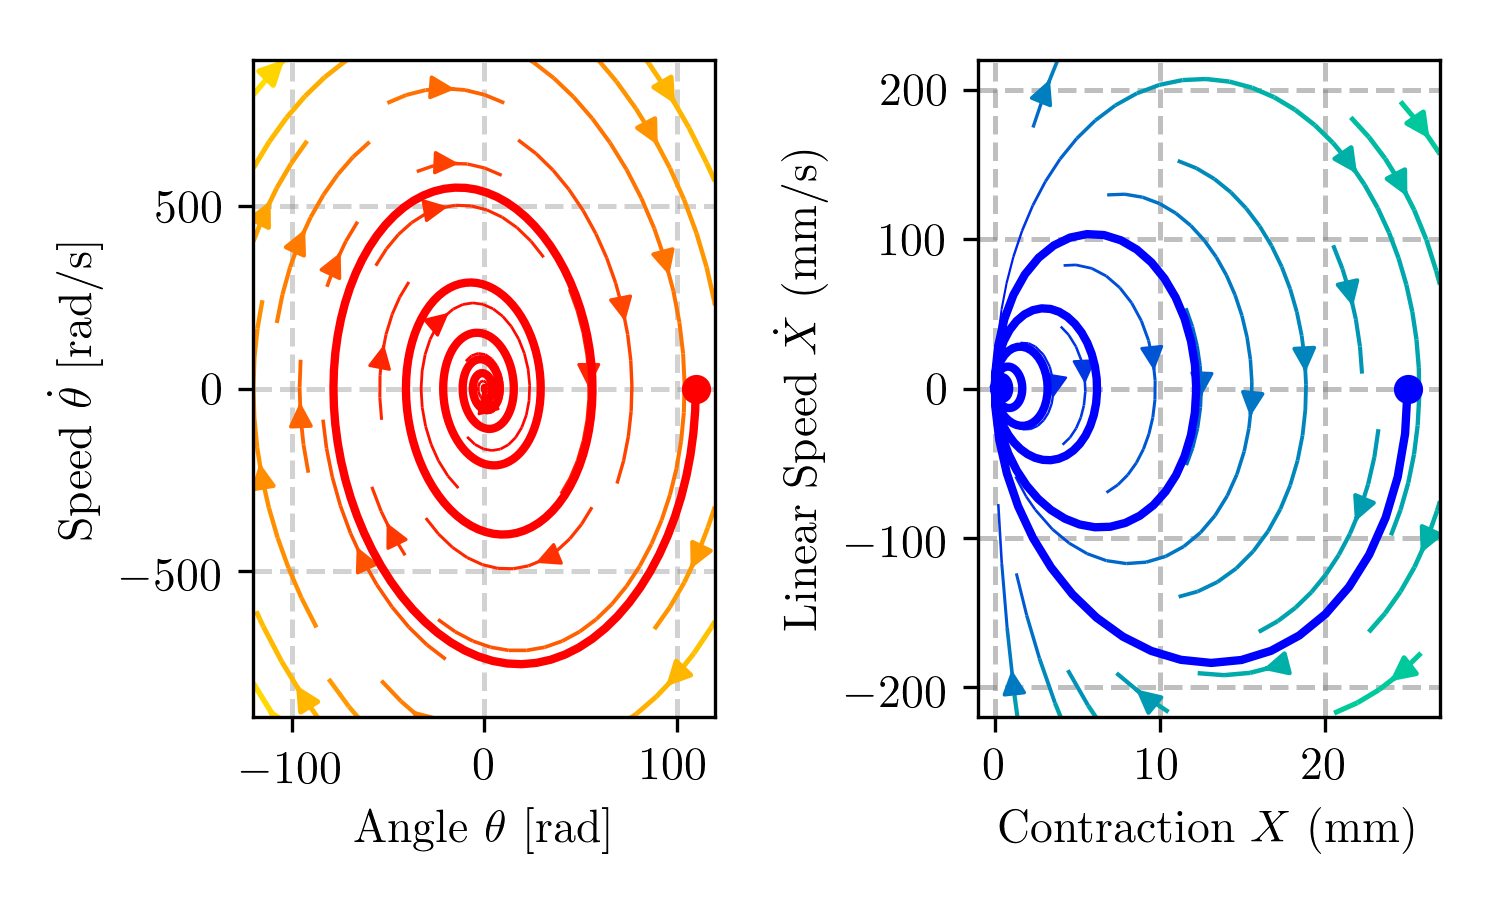
\includegraphics[trim= 0.0cm 0.8cm 0.0cm 0.0cm,width=1.0\columnwidth]{pics/plots/phase_space_model.png}
		\caption{Phase plots of damped oscillations in a TSA system in the motor (left) and payload (right) coordinates. Vector fields indicate the direction of motion in various points of the phase plot}
 		\label{fig:phase_plots_simulation}
		\vspace*{-2mm} 
\end{figure}

As the next step, we have decided to repeat the simulations whose results are presented in Fig. \ref{fig:energies_simulation} and \ref{fig:phase_plots_simulation} on a practical setup, and the experimental evaluation is described in the next section. 



